%-------------------------------------------------------------------------------
%-------------------------------------------------------------------------------
%-------------------------------------------------------------------------------
\chapter{Listes dynamiques}
%-------------------------------------------------------------------------------
%-------------------------------------------------------------------------------
\thispagestyle{empty}

\vskip -2cm
%-------------------------------------------------------------------------------
%-------------------------------------------------------------------------------
{\sf Dans ce T.P. nous allons utiliser utiliser le caractère dynamique des listes python.

On peut construire sans connaître à l'avance la taille de la liste.

Une première conséquence est qu'il est possible de construire une liste de taille $n$ en partant d'une liste vide et y adjoignant $n$ éléments. On a maintenant deux possibles pour construire une liste de taille donnée, la construction avec \type{append} étant légèrement plus lente.
% \begin{lstlisting}
% def f1(n):                      def f2(n):
%     L = [0]*n                       L = []    
%     for i in range(n):              for i in range(n):
%         L[i] = fonction(i)              L.append(fonction(i)
%     return L                        return L
% \end{lstlisting}

On pourra tester les fonctions avec la liste 
\begin{lstlisting}
Ex = [ 0, -2,  1, -2, -2, -1,  2,  3,  3,  0,
       0,  0,  1,  2,  0, -2, -1, -1,  1,  3,
       3,  1,  3,  0,  2, -1, -1,  1,  1,  1 ]
\end{lstlisting}
}
%-------------------------------------------------------------------------------
%-------------------------------------------------------------------------------
%-------------------------------------------------------------------------------
\section{Exercices} 
%-------------------------------------------------------------------------------
%-------------------------------------------------------------------------------
%-------------------------------------------------------------------------------
\begin{Exercise}[title = Termes positifs]
\it Écrire une fonction \type{positifs(L)} qui renvoie la liste des termes strictement positifs de \type{L}, dans le même ordre.

\type{positifs(Ex)} renvoie \type{[1, 2, 3, 3, 1, 2, 1, 3, 3, 1, 3, 2, 1, 1, 1]}
\end{Exercise}
%-------------------------------------------------------------------------------
\begin{Answer}
\begin{lstlisting}
def positifs(L):
    pos = []
    for x in L:
        if x > 0:
           pos.append(x)
    return pos
\end{lstlisting}

Python propose aussi la construction
\begin{lstlisting}
[x for x in L if x >=0]
\end{lstlisting}

\end{Answer}
%-------------------------------------------------------------------------------
%-------------------------------------------------------------------------------
\begin{Exercise}[title = Recherche, label = exo:positions]
\it Écrire une fonction \type{positions(x, L)} qui renvoie la liste des indices $i$ en lesquels \type{L[i]} vaut $x$, la liste renvoyée sera vide si $x$ n'apparaît pas dans la liste.

\type{positions(-1, Ex)} renvoie \type{[5, 16, 17, 25, 26]}
\end{Exercise}
%-------------------------------------------------------------------------------
\begin{Answer}
\begin{lstlisting}
def positions(x, L):
    n = len(L)
    pos = []
    for i in range(n):
        if L[i] == x:
           pos.append(i)
    return pos
\end{lstlisting}

\begin{lstlisting}
[i for i in range(len(L)) if L[i] == x]
\end{lstlisting}
\end{Answer}
%-------------------------------------------------------------------------------
%-------------------------------------------------------------------------------
\begin{Exercise}[title = Positions du maximum]
\it Écrire une fonction \type{indices\_max(L)} qui renvoie la liste des indices $i$ en lesquels \type{L[i]} vaut le maximum de la liste. On pourra, dans un premier temps, utiliser l'exercice {\bf \ref{exo:positions}} après avoir calculé la valeur du maximum. Il existe cependant une méthode qui permet de trouver le résultat en ne parcourant qu'une fois la liste.

\type{indices\_max(Ex)} renvoie \type{[7, 8, 19, 20, 22]}
\end{Exercise}
%-------------------------------------------------------------------------------
\begin{Answer}
La méthode naturelle
\begin{lstlisting}
def indices_max(L):
    maxi = L[0]
    for x in L:
        if x > maxi:
            maxi = x
    return positions(maxi, L)
\end{lstlisting}

En un seul passage
\begin{lstlisting}
def indices_max(L):
    n = len(L)
    maxi = L[0]
    pos = [0]
    for i in range(1, n):
        if L[i] > maxi:
            maxi = L[i]
            pos = [i]
        elif L[i] == maxi:
            pos.append(i)
    return pos
\end{lstlisting}

\newpage
\end{Answer}
%-------------------------------------------------------------------------------
%-------------------------------------------------------------------------------
\begin{Exercise}[title = Doublons]
\it Écrire une fonction \type{sans\_doublon(L)} qui renvoie la liste des valeurs de \type{L} dans le même ordre mais sans répétitions dans des termes consécutifs.

\type{sans\_doublon(Ex)} renvoie 

\type{[0, -2, 1, -2, -1, 2, 3, 0, 1, 2, 0, -2, -1, 1, 3, 1, 3, 0, 2, -1, 1]}
\end{Exercise}
%-------------------------------------------------------------------------------
\begin{Answer}
On n'ajoute un élément que s'il est distinct de son prédécesseur, le premier terme n'a pas à être comparé.
\begin{lstlisting}
def sans_doublon(L):
    n = len(L)
    L1 = [L[0]]
    for i in range(1, n):
        if L[i] != L[i-1]:
            L1.append(L[i])
    return L1
\end{lstlisting}
\end{Answer}
%-------------------------------------------------------------------------------
%-------------------------------------------------------------------------------
%-------------------------------------------------------------------------------
\section{Complément : parenthésage} 
%-------------------------------------------------------------------------------
%-------------------------------------------------------------------------------
%-------------------------------------------------------------------------------
On veut étudier le parenthésage d'expressions arithmétiques ou du code source d'un programme. Il est utile de déterminer la parenthèse ouvrante associée à une parenthèse fermante, les éditeurs montrent souvent les appariements  de parenthèses.
%-------------------------------------------------------------------------------
\begin{center}
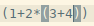
\includegraphics{TP10_parentheses.png}
\end{center}
%-------------------------------------------------------------------------------

Par exemple dans $1 + 2*(7-(4-3)*((2-5)+2*((12/4-8)+2*3)))$la parenthèse ouvrante après $(4-3)*$ est associée à l'avant dernière parenthèse fermante.

On considère une chaîne de caractère représentant l'expression et on s'intéresse uniquement aux parenthèses classiques "(" et ")". On rappelle qu'une chaîne de caractères se manipule comme si elle était une liste de caractères, avec la particularité qu'elle n'est pas modifiable.
%-------------------------------------------------------------------------------
%-------------------------------------------------------------------------------
\begin{Exercise}[title = {Test de parenthésage}]\it

Écrire une fonction \type{testPar(ch)} pour qu'elle renvoie \type{True} ou \type{False} selon que la chaîne de caractères est bien parenthésée ou non.
\end{Exercise} 
%-------------------------------------------------------------------------------
\begin{Answer}

Il suffit de compter le nombre de parenthèses ouvrantes non encore fermées.

Un manque de parenthèses ouvrantes se voit quand ce nombre est nul alors qu'on lit une parenthèse fermante, un excès de parenthèses ouvrantes se voit à la fin si le nombre est non nul.
\begin{lstlisting}
def testPar(ch):
    n = len(ch)
    ouv = 0
    for i in range(n):
        car = ch[i]
        if car == "(":
            ouv = ouv + 1
        if car == ")":
            if ouv == 0:
                return False
            else:
                ouv = ouv - 1
    return ouv == 0
\end{lstlisting}
\end{Answer}
%-------------------------------------------------------------------------------
%-------------------------------------------------------------------------------
Pour associer une parenthèse fermante à la parenthèse ouvrante associée, on peut remarquer que celle-ci est la dernière parenthèse ouvrante non encore associée. Pour la calculer on peut appliquer l'algorithme suivant

\begin{itemize}
\item On crée une liste vide pour les couples de parenthèses, \type{par}.
\item On crée une liste vide pour les indices de parenthèses ouvrantes, \type{ouv}.
\item On lit les caractères un par un,
\begin{itemize}
\item quand on voit une parenthèse ouvrante on ajoute (\type{ouv.append}) sa position,
\item quand on lit une parenthèse fermante à la position $j$,  on enlève (\type{ouv.pop}) la dernière valeur depuis la liste \type{ouv}, $i$,  ce sera bien la dernière parenthèse ouvrante non encore associée ; on ajoute alors (\type{par.append}) le couple $(i, j)$ à la liste \type{par}.
\end{itemize}
\end{itemize}

Dans la chaîne \type{"1+2*(7-(4-3)*((2-5)+2*((12/4-8)+2*3)))"} les opérations  seront 

\begin{center}
\begin{tabular}{r|c|l|l}
chaîne lue&$i$&\type{ouv}&\type{par} \\
\hline
\type{"1"}&0&\type{[]}&\type{[]}\\
\type{"1+2*("}&4&\type{[4]}&\type{[]}\\
\type{"2*(7-("}&7&\type{[4, 7]}&\type{[]}\\
\type{"-(4-3)"}&11&\type{[4]}&\type{[(7, 11)]}\\
\type{"...)*("}&13&\type{[4, 13]}&\type{[(7, 11)]}\\
\type{"...*(("}&14&\type{[4, 13, 14]}&\type{[(7, 11)]}\\
\type{"...-5)"}&18&\type{[4, 13]}&\type{[(7, 11), (14, 18)]}\\
\type{"...2*("}&22&\type{[4, 13, 22]}&\type{[(7, 11), (14, 18)]}\\
\type{"...*(("}&23&\type{[4, 13, 22, 23]}&\type{[(7, 11), (14, 18)]}\\
\type{"...-8)"}&30&\type{[4, 13, 22]}&\type{[(7, 11), (14, 18), (23, 30)]}\\
\type{"...*3)"}&35&\type{[4, 13]}&\type{[(7, 11), (14, 18), (23, 30), (22, 35)]}\\
\type{"...3))"}&36&\type{[4]}&\type{[( 7, 11), (14, 18), (23, 30), ...}\\
               &  &          &\type{ (22, 35), (13, 36)]}\\
\type{"...)))"}&37&\type{[]}&\type{[( 7, 11), (14, 18), (23, 30), ...}\\
               &  &         &\type{ (22, 35), (13, 36), ( 4, 37)]}\\
\end{tabular}
\end{center}
%-------------------------------------------------------------------------------
%-------------------------------------------------------------------------------
\begin{Exercise}[title = {Liste des parenthèses associées}]\it

Écrire une fonction \type{listePar(ch)} qui reçoit une chaîne de caractères {\bf supposée bien parenthésée} et qui retourne la liste des couples d'indices de parenthèses associées.
\end{Exercise} 
%-------------------------------------------------------------------------------
\begin{Answer}
\begin{lstlisting}
def listePar(ch):
    n = len(ch)
    par = []
    ouv = []
    for i in range(n):
        car = ch[i]
        if car == "(":
            ouv.append(i)
        if car == ")":
            j = ouv.pop()
            par.append((j, i))
    return par
\end{lstlisting}

\newpage
\end{Answer}
%-------------------------------------------------------------------------------
%-------------------------------------------------------------------------------
\begin{Exercise}[title = {Test de parenthésage bis}]\it

Écrire une fonction \type{mauvaisePar(ch)} pour qu'elle renvoie \type{-1} si la chaîne est bien parenthésée ou bien un indice $i$ indiquant la position d'une parenthèse ouvrante non fermée ou la position d'une parenthèse fermante sans parenthèse ouvrante associée.

Par exemple \type{listePar("(1+2))*(5-3)")} renvoie \type{5}.
\end{Exercise} 
%-------------------------------------------------------------------------------
\begin{Answer}

Il suffit de compter le nombre de parenthèses ouvrantes non encore fermées.

Un manque de parenthèses ouvrantes se voit quand ce nombre est nul alors qu'on lit une parenthèse fermante, un excès de parenthèses ouvrantes se voit à la fin si le nombre est non nul.
\begin{lstlisting}
def mauvaisePar(ch):
    n = len(ch)
    ouv = []
    for i in range(n):
        car = ch[i]
        if car == "(":
            ouv.append(i)
        if car == ")":
            if ouv == []:
                return i
            else:
                j = ouv.pop()
    if ouv == []:
        return -1
    else:
        return ouv.pop()
\end{lstlisting}

On peut aussi renvoyer toutes les paires de parenthèses, y comprises celles qui ne sont pas appariées, en indiquant avec \type{-1} la parenthèses manquante.

\begin{lstlisting}
def parentheses(ch):
    n = len(ch)
    par = []
    ouv = []
    for i in range(n):
        car = ch[i]
        if car == "(":
            ouv.append(i)
        if car == ")":
            if ouv == []:
                par.append((-1, i))
            else:
                j = ouv.pop()
                par.append((j, i))
    while ouv != []:
        i = ouv.pop()
        par.append((i, -1))
    return par
\end{lstlisting}

\end{Answer}
%-------------------------------------------------------------------------------
%-------------------------------------------------------------------------------

